\input{../header}
\usetikzlibrary{shapes.geometric}

\begin{document}
%


%\onehalfspacing
\allowdisplaybreaks
%##################################################################
\section{Related rates recipe}
A lot of calculus students find related rates (and applied optimization) particularly tricky, and here's why: \textit{there's no formula for doing them.} Every situation is a bit different, and what works in one case doesn't necessarily work in another.

There is, however, a \textit{recipe} (if I was feeling very fancy I would call it a \textit{heuristic} -- google it) that you can follow to think your way through related rates problems.

\begin{enumerate}
    \item Draw three pictures.
    \begin{itemize}
        \item I mean it. If you don't draw three, it's harder to see what's changing.
        \item Draw your pictures pretty big, or you'll have a hard time labeling.
    \end{itemize}
    \item Determine what quantities are \textit{changing} (ie., variables) and what ones are staying the same.
    \begin{itemize}
        \item If something is changing, label it with a letter.
        \item If something is staying the same, label it with what number it is.
    \end{itemize}
    \item Write down what you know and what you want to know.
    \begin{itemize}
        \item Use good derivative grammar, \(\dfrac{d\square}{dt}\), to label any rates.
        \item Make a note of what things are \textit{always} true and what things are only true \textit{sometimes.}
    \end{itemize}
    \item Write down an equation relating the variables.
    \begin{itemize}
        \item Creativity! Geometry! Trigonometry! Other math you remember!
    \end{itemize}
    \item Find the derivative, \textit{\textbf{with respect to time!!}}, of both sides.
    \begin{itemize}
        \item Remember, all of your variables are secretly some weird function of time.
        \item You have now \textit{related} the \textit{rates}!
    \end{itemize}
    \item Substitute in the values you know; solve for the rate you want.

\end{enumerate}

The best way to learn related rates problems is to do a hundred related rates problems. Guess what we're about to do?

\pagebreak

\section{PS9: Related rates}


\everymath{\displaystyle}
\begin{enumerate}[leftmargin=0pt]

\item Beer is often brewed in big tanks where the bottom is a circular cone pointing down. We're going to just focus on the cone part; let's say that the top radius of the cone is 6 feet and the depth of the cone is 8 feet. 

If I am pumping the water out of the tank at a rate of \(4 \text{ ft}^3 / \text{ min}\), how fast is the water level falling when the water in the tank is 3 feet deep?

\item A television camera is positioned 4000 feet away from the base of a rocket launching pad. As the rocket goes up, the camera has to tilt up to keep the rocket in frame. In addition, the auto-focus of the camera has to take into account the increasing distance between the camera and the rocket.
\begin{enumerate}
    \item Suppose that the rocket's speed is 600 ft / sec at the moment it is 3000 feet off the ground. How fast is the camera's tilt angle changing at that same moment?
    \item How fast is the distance from the camera to the rocket changing at that same moment?
\end{enumerate}

\item A skateboarder who is 6 feet tall rides past a 15 foot tall lamppost. As he gets further from the lamppost, his shadow gets longer. 

If he is riding at a constant speed of 3 ft / sec, how fast is the length of his shadow growing at the moment he is 8 feet away from the lamppost?

\item 
\begin{multicols}{2}
A baseball diamond is a big square that is 90 feet on each side (see the diagram on the right). 

A batter hits a ball along the line from third base to home plate and runs toward first base. 
\vfill
\begin{center}
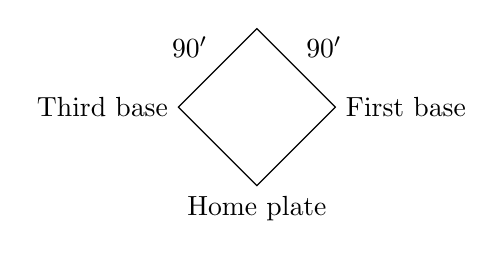
\begin{tikzpicture}
    \node[diamond, draw, minimum height=2cm, minimum width=2cm] (d) at (0, 0) {}; 
    \node[below] (home) at (d.south) {Home plate};
    \node[right] (1b) at (d.east) {First base};
    \node[left] (3b) at (d.west) {Third base};
    \node[above right] (1b2b) at (d.45) {$90'$};
    \node[above left] (2b3b) at (d.135) {$90'$};
\end{tikzpicture}
\end{center}
\end{multicols}
\begin{enumerate}
    \item How fast is the distance between the ball and first base changing when the ball is halfway to third base, if at that instant the ball is traveling 100 ft / sec?
    \item How fast is the distance between the ball and the runner changing at the same instant, if at the same instant the runner is 10 feet away from home plate, running at 30 ft / sec?
\end{enumerate}

\item A boat is being pulled towards a dock using a long rope.  One end of the rope is attached to the boat 3 feet above the water; the other end is attached to a winch (a machine that winds up rope) at a height of 10 feet above the water. 

When the boat is still 12 feet from the dock, the rope is getting pulled in at a rate of 3 inches per second (that's 0.25 ft / sec). How fast is the boat traveling at this time?

\item While Violet Beauregarde is at Willy Wonka's Chocolate Factory, she snatches some experimental gum against Wonka's warnings. Not yet perfected, the gum has the side effect of expanding Violet into a giant human blueberry. At one point, after she becomes perfectly spherical, she reaches a volume of $1.8\text{ m}^3$ and is still growing at $0.2 \text{ m}^3/\text{ s}$. 
\begin{enumerate}
    \item How fast is her radius increasing? 
    \item How fast is her surface area increasing?
\end{enumerate}
\end{enumerate}
\end{document}